% ======================================
%            CyberEdu QUIZZ
%            VOLUME 1
%            Mise en forme Moodle QUIZZ
%            (c) eric.dupuis@lecnam.net
% ======================================
\documentclass[12pt]{article}

%  \usepackage[draft]{moodle}
   \usepackage{moodle}
   \usepackage{moodle}
\usepackage{graphicx}
\usepackage{xpatch}

\makeatletter
\def\graphicspath#1{\def\Ginput@path{#1}\edef\moodleimgpath{\@firstofone#1}}
%

\xpatchcmd{\moodle@includegraphics@int@int}%
{\openssl\otherspace enc -base64 -in \moodleimgpath#2.png -out #2.enc}%
{\openssl\otherspace enc -base64 -in \moodleimgpath#2.png -out #2.enc}%
{\typeout{patch ok}}%
{\typeout{patch failed}}
\makeatother

\graphicspath{{./img/}}

   \begin{document}

% =====================================
   \begin{quiz}{CYBERDEF101-Cyberedu-QUIZZ 3}
% =====================================


% Q.........................................
\begin{multi}[multiple=true]{Cyberedu-QUIZZ-ID-3.1}
	La s\'ecurit\'e est au coeur de l'impl\'ementation de la famille de protocoles IP:
\item Vrai
\item* Faux
\end{multi}
% Q.........................................
\begin{multi}[multiple=true]{Cyberedu-QUIZZ-ID-3.2}
	Lors de l'utilisation du protocole IP, il est nativement possible d'authentifier les \'emetteurs et r\'ecepteurs d'un datagramme IP:
\item Vrai
\item* Faux
\end{multi}
% Q.........................................
\begin{multi}[multiple=true]{Cyberedu-QUIZZ-ID-3.3}
	Le chiffrement des donn\'ees transport\'ees est automatiquement pris en compte dans la famille de protocole IP au niveau de la couche de Transport:
\item Vrai
\item* Faux
\end{multi}
% Q.........................................
\begin{multi}[multiple=true]{Cyberedu-QUIZZ-ID-3.4}
	Lorsqu'un attaquant C peut \'ecouter et modifier les informations \'echang\'ees entre A et B, on parle d'\'ecoute  :
\item Passive
\item* Active
\item Hacktiviste
\item Discr\`ete
\end{multi}
% Q.........................................
\begin{multi}[multiple=true]{Cyberedu-QUIZZ-ID-3.5}
	Entourer au moins 2 m\'ecanismes de s\'ecurit\'e compl\'ementaires pouvant servir \`{a} s\'ecuriser les r\'eseaux sur IP
\item L'utilisation d'Internet
\item* Le chiffrement des communications
\item* Le cloisonnement des r\'eseaux
\item* L'authentification des entit\'es
\end{multi}
% Q.........................................
\begin{multi}[multiple=true]{Cyberedu-QUIZZ-ID-3.6}
	Entourer 2 m\'ecanismes/technologies qui peuvent servir \`{a} s\'ecuriser les r\'eseaux sur IP
\item* Le filtrage des flux
\item* La supervision des \'equipements
\item L'usage des r\'eseaux sans fil, comme le Wifi
\item Le BYOD (Bring your Own Device)
\end{multi}
% Q.........................................
\begin{multi}[multiple=true]{Cyberedu-QUIZZ-ID-3.7}
	Entourer un \'equipement qui permet de d\'efinir et contr\^oler les flux autoris\'es et interdits entre deux r\'eseaux ? (Slide Pare-feu)
\item Un routeur
\item* Un pare-feu
\item Un hub
\item Un r\'epartiteur de charge
\end{multi}
% Q.........................................
\begin{multi}[multiple=true]{Cyberedu-QUIZZ-ID-3.8}
	Quel r\^ole un proxy (serveur mandataire) peut-il jouer en mati\`ere de s\'ecurit\'e? (Slide Pare-feu : 13)
\item Il peut mettre en cache des pages Internet d\'ej\`{a} demand\'ees.
\item* Il peut autoriser ou interdire certains flux applicatifs.
\item Il peut rechercher des \'el\'ements malveillants
\item Il peut chiffrer les communications
\end{multi}
% Q.........................................
\begin{multi}[multiple=true]{Cyberedu-QUIZZ-ID-3.9}
	Quel \'equipement peut aider \`{a} se prot\'eger des d\'enis de services distribu\'es? (Slide 14 : R\'epartiteur de charge)
\item Un antivirus
\item Un routeur
\item Un proxy
\item* Un r\'epartiteur de charge
\end{multi}
% Q.........................................
\begin{multi}[multiple=true]{Cyberedu-QUIZZ-ID-3.10}
	Mon antivirus me prot\`ege suffisamment. Je suis \`{a} l'abri de tous les virus, y compris des virus \`{a} paraitre non encore d\'etect\'es (0-day)? (Slide Antivirus : 16)
\item Vrai
\item* Faux
\end{multi}
% Q.........................................
\begin{multi}[multiple=true]{Cyberedu-QUIZZ-ID-3.11}
	Quel \'el\'ement composant l'antivirus lui permet de d\'etecter les codes malveillants connus?  (Slide 16 : Antivirus)
\item Le nom de l'\'editeur (Sophos, Trend Micro, McAfee, …)
\item La matrice de flux
\item* La base de donn\'ees des signatures
\item Le moteur de chiffrement
\end{multi}
% Q.........................................
\begin{multi}[multiple=true]{Cyberedu-QUIZZ-ID-3.12}
	Quel \'equipement r\'eseau peut \^etre utilis\'e pour d\'etecter une intrusion? (Slide 18 : IDS et IPS)
\item Un pare-feu
\item* Un IDS
\item Un IPS
\item Un antivirus
\end{multi}
% Q.........................................
\begin{multi}[multiple=true]{Cyberedu-QUIZZ-ID-3.13}
	Quelle technologie permet de cr\'eer une communication (tunnel) s\'ecuris\'ee entre deux r\'eseaux en s'appuyant sur un r\'eseau qui n'est pas de confiance? (Slide 20 : VPN)
\item Internet
\item Wifi
\item* VPN
\item 4G
\end{multi}
% Q.........................................
\begin{multi}[multiple=true]{Cyberedu-QUIZZ-ID-3.14}
	Entourer les bonnes r\'eponses.  Un VPN TLS est un tunnel est \'etabli au niveau de la couche de  : (Slide 22 : VPN)
\item Donn\'ees
\item IP
\item* Transport
\item Https
\end{multi}
% Q.........................................
\begin{multi}[multiple=true]{Cyberedu-QUIZZ-ID-3.15}
	La cryptographie est seul moyen de cr\'eer des VPN de mani\`ere s\'ecuris\'ee: (Slide 23 : VPN)
\item Vrai
\item* Faux
\end{multi}
% Q.........................................
\begin{multi}[multiple=true]{Cyberedu-QUIZZ-ID-3.16}
	Les VLAN sont des r\'eseaux virtuels impl\'ement\'es sur les routeurs: (Slide 26 : Segmentation)
\item Vrai
\item* Faux
\end{multi}
% Q.........................................
\begin{multi}[multiple=true]{Cyberedu-QUIZZ-ID-3.17}
	Un proxy me permet de masquer mon adresse interne vis-\`{a}-vis d'Internet: (Slide 37 : Exemple pratique de s\'ecurisation avec un r\'eseau simple)
\item* Vrai
\item Faux
\end{multi}
% Q.........................................
\begin{multi}[multiple=true]{Cyberedu-QUIZZ-ID-3.18}
	Dans les r\`egles de bonnes pratiques, les \'equipements qui communiquent directement avec Internet doivent \^etre mis dans une DMZ : (Slide 37 : Exemple pratique de s\'ecurisation avec un r\'eseau simple)
\item* Vrai
\item Faux
\end{multi}
% Q.........................................
\begin{multi}[multiple=true]{Cyberedu-QUIZZ-ID-3.19}
	Comment s'appelle le processus de transformation d'un texte  en clair   en un  texte illisible  \`{a} l'aide d'un algorithme? (Slide 42 : Vocabulaire)
	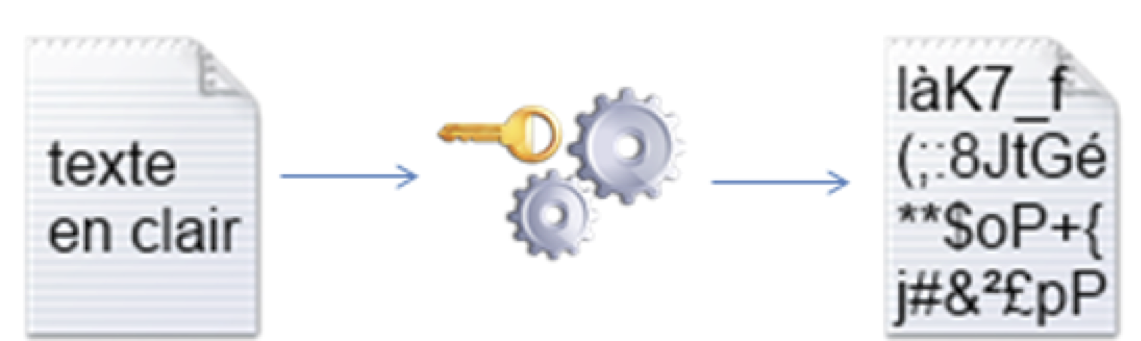
\includegraphics[width=6cm]{img/img3-19}
\item* Le chiffrement
\item Le cryptage
\item La signature
 \end{multi}
% Q.........................................
\begin{multi}[multiple=true]{Cyberedu-QUIZZ-ID-3.20}
	Lorsque la cl\'e utilis\'ee pour transformer un texte  en clair  en texte illisible est la m\^eme pour rendre, le texte  illisible  en texte  en clair , on parle de ? (Slide 50 : Chiffrement sym\'etrique)
	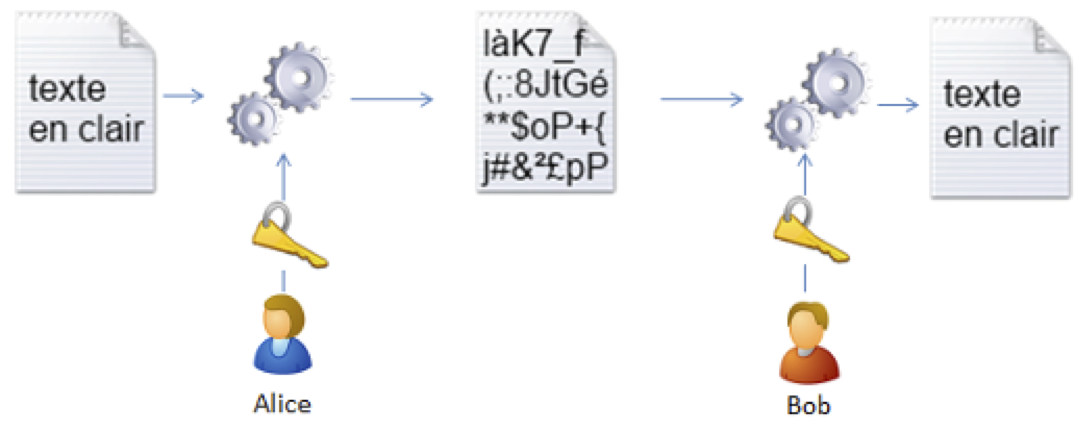
\includegraphics[width=6cm]{img/img3-20}
\item Cloisonnement
\item Chiffrement asym\'etrique
\item* Chiffrement sym\'etrique
\item Virtualisation
 \end{multi}
% Q.........................................
\begin{multi}[multiple=true]{Cyberedu-QUIZZ-ID-3.21}
	Lorsque pour envoyer un message priv\'e \`{a} Bob, Alice utilise la cl\'e  publique de Bob pour rendre   illisible  le  texte en clair , et que Bob utilise sa cl\'e priv\'ee pour transformer le texte  illisible  en   texte en clair , on parle de ? (Slide 52 : Chiffrement asym\'etrique)
		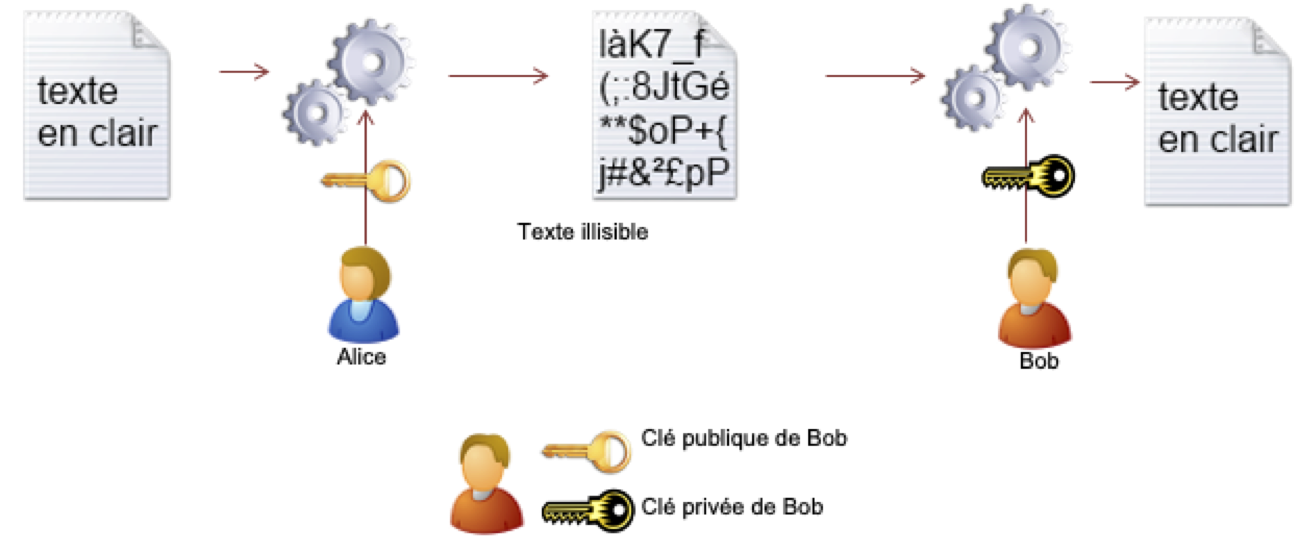
\includegraphics[width=6cm]{img/img3-21}
\item Chiffrement sym\'etrique
\item Tokenisation
\item Envoi priv\'e
\item* Chiffrement asym\'etrique
\end{multi}
% Q.........................................
\begin{multi}[multiple=true]{Cyberedu-QUIZZ-ID-3.22}
	Consid\'erant les besoins de s\'ecurit\'e, entourer le(s) besoin(s) assur\'e(s) par la signature \'electronique : (Slide 54 : Signature \'electronique)
\item Disponibilit\'e,
\item* Int\'egrit\'e
\item Confidentialit\'e
\item Suret\'e
\end{multi}
% Q.........................................
\begin{multi}[multiple=true]{Cyberedu-QUIZZ-ID-3.23}
	Entourer les \'el\'ements qu'on peut retrouver dans un certificat \'electronique d'une entit\'e: (Slide 61 : Certificats \'electroniques)
\item* Les noms, pr\'enoms, URL de l'entit\'e (ou son url)
\item La cl\'e priv\'ee de l'entit\'e
\item* La signature d'un tiers de confiance (des autorit\'es de certification)
\item* La p\'eriode de validit\'e du certificat
\end{multi}
% Q.........................................
\begin{multi}[multiple=true]{Cyberedu-QUIZZ-ID-3.24}
	Lors de la navigation sur Internet, les  fichiers temporaires cr\'e\'es et g\'er\'es par les navigateurs Web afin de stocker les informations concernant les utilisateurs telles que : (Slide 67 : Usurpation d'identit\'e via les cookies), (Son identifiant, Les th\`emes et les pr\'ef\'erences d'affichage) sont appel\'es
\item les logs
\item La cl\'e priv\'ee de l'entit\'e
\item les fichiers INI
\item* les cookies
\end{multi}
% Q.........................................
\begin{multi}[multiple=true]{Cyberedu-QUIZZ-ID-3.25}
	Depuis Internet, lorsqu'un attaquant r\'eussit \`{a} contourner les m\'ecanismes d'authentification et \`{a} interroger directement la base de donn\'ees  par \'ecriture de commandes sp\'ecifiques on parle de (Slide 72 : Injection SQL)
\item Hacking
\item XSS (Cross Site Scripting)
\item* Injection SQL
\item Malware
\end{multi}
% Q.........................................
\begin{multi}[multiple=true]{Cyberedu-QUIZZ-ID-3.26}
	Lors de la navigation en https sur un site Web, entourer les propositions ci-dessous qui sont vraies: (Slide 63 : Certificats \'electroniques)
\item* Le site web dispose d'un certificat \'electronique
\item* Tous les \'echanges entre le site Web et mon navigateur doivent \^etre chiffr\'es
\item Tous les \'echanges entre le site Web et mon navigateur sont analys\'es par mon antivirus
\item Le d\'ebit des communications Internet est plus rapide
\end{multi}
% Q.........................................
\begin{multi}[multiple=true]{Cyberedu-QUIZZ-ID-3.27}
	Lors de la navigation en https sur un site Web, il faut faire attention \`{a} :
\item* La validit\'e du certificat annonc\'e par le site (le certificat n'a pas encore expir\'e)
\item* L'autorit\'e ayant accord\'e le certificat (par exemple, il ne faudrait que le certificat soit auto-sign\'e ou issue d'une autorit\'e non reconnue)
\item* L'alerte de mon navigateur indiquant que le certificat pr\'esent\'e par le site n'est pas de confiance
\item Il n'y pas de raison de faire attention,  https  signifie que je peux naviguer en toute confiance.
\end{multi}


  \end{quiz}
   \end{document}
